\documentclass[../main.tex]{subfiles}
\begin{document}

\begin{definition}\label{def:3.6.1}
    设二维随机向量 $(X,Y)$ 的 CDF 为 $F(x,y)$,若 $F(x,y)=F_X(x)F_Y(y),\forall x,y\in\mathbb R$,则称 $X,Y$ 相互\emph{独立}。
\end{definition}

可以证明,对于二维离散型(或连续型)随机向量 $(X,Y)$,$X,Y$ 相互独立的充要条件是 $f(x,y)=f_X(x)f_Y(y),\forall x,y\in\mathbb R$,其中 $f(x,y)$ 为联合 PMF(或 PDF)。

\begin{definition}\label{def:3.6.2}
    设 $n$ 维随机向量 $(X_1,\cdots,X_n)$ 的 CDF 为 $F(x_1,\cdots,x_n)$,若 $F(x_1,\cdots,x_n)=F_{1}(x_1)\cdots F_n(x_n),\forall x_1,\cdots,x_n\in\mathbb R$,则称 $X_1,\cdots,X_n$ 相互\emph{独立}。
\end{definition}

可以证明,对于 $n$ 维离散型(或连续型)随机向量 $(X_1,\cdots,X_n)$,$X_1,\cdots,X_n$ 相互独立的充要条件是 $f(x_1,\cdots,x_n)=f_1(x_1)\cdots f_n(x_n),\forall x_1,\cdots,x_n\in\mathbb R$,其中 $f(x_1,\cdots,x_n)$ 为联合 PMF(或 PDF)。

\begin{theorem}\label{thm:3.6.1}
    \mbox{}
    \begin{enumerate}
        \item 若 $X_1,\cdots,X_n$ 相互独立,则 $\forall m\in\{1,\cdots,n-1\}$,可测函数 $g_1,g_2$,有 $Y_1=g_1(X_1,\cdots,X_m)$ 与 $Y_2=g_2(X_{m+1},\cdots,X_n)$ 相互独立。
        \item 若 $n$ 维连续型随机向量 $(X_1,\cdots,X_n)$ 的联合 PDF 满足
              \begin{equation*}
                  f(x_1,\cdots,x_n)=g_1(x_1)\cdots g_n(x_n),\forall x_1,\cdots,x_n\in\mathbb R,
              \end{equation*}
              其中 $g_i:\mathbb R\rightarrow [0,+\infty),\forall i\in\{1,\cdots,n\}$,则 $X_1,\cdots,X_n$ 相互独立,且 $X_i$ 的边际 PDF $f_i$ 与 $g_i$ 相差常数因子,$\forall i\in\{1,\cdots,n\}$。
    \end{enumerate}
\end{theorem}

\begin{example}
    设 $(X,Y)$ 服从如图~\ref{fig:3.6.1} 的三角形域 $D$ 上的均匀分布,即 $
        f(x,y)=\left\{
        \begin{aligned}
            c & , & (x,y)\in D,  \\
            0 & , & \text{其他},
        \end{aligned}
        \right.
    $ 则 $X,Y$ 不独立。

    \begin{figure}[!h]
        \centering
        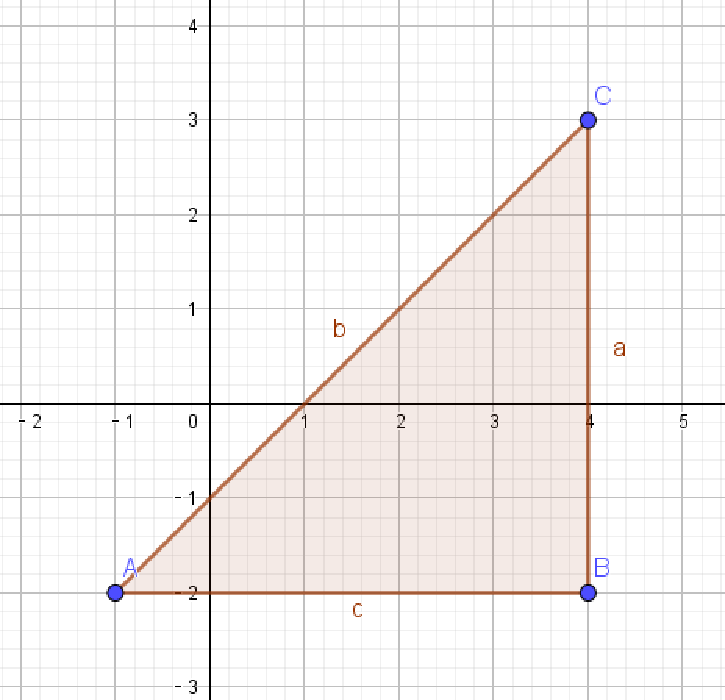
\includegraphics[scale=0.4]{figures/triangle.pdf}
        \caption{三角形域上的均匀分布}
        \label{fig:3.6.1}
    \end{figure}
\end{example}

\end{document}
